% !TeX spellcheck = cs_CZ
%{\tikzset{external/prefix={tikz/FYZII/}}
% \tikzset{external/figure name/.add={ch14_}{}}
%---------------------------------------------------------------------------------------------------
% file fey2ch14.tex
%---------------------------------------------------------------------------------------------------
%====================Kapitola: Magnetické pole v různých případech =================================
\setchaptertoc
\chapter{Magnetické pole v různých případech}\label{fyz:IIchapXIV}
  \section{Vektorový potenciál}\label{fyz:IIchapXIVsecI}
    V této kapitole budeme pokračovat v diskuzi o magnetických polích podmíněných stacionární mi
    proudy, což je předmětem magnetostatiky. Magnetické pole souvisí s elektrickými proudy
    prostřednictvím základních rovnic
    \begin{subequations}\label{fyz:eq1006}
      \begin{align}
        \ndiver{B}   &= 0                                      \label{fyz:eq1006a}  \\
        c^2\nrot{B}  &= \dfrac{\vec{j}}{\varepsilon_0}         \label{fyz:eq1006b}
      \end{align}
    \end{subequations}

    Chtěli bychom tyto rovnice vyřešit nejobecnějším matematickým způsobem, tedy bez požadavku
    speciální symetrie nebo intuitivního odhadu. V elektrostatice jsme našli přímý způsob určování
    pole, jsou-li známy polohy všech elektrických nábojů: Vypočte se skalární potenciál \(\varphi\)
    tak, že se integruje přes všechny náboje jako v rovnici \eqref{fyz:eq1007b}. Elektrické pole se
    potom určí tak, že potenciál \(\varphi\) zderivujeme. Ukážeme, že existuje analogický postup
    určení magnetického pole \(\vec{B}\) v němž je třeba znát proudovou hustotu \(\vec{j}\) všech
    pohybujících se nábojů.

    Viděli jsme, že v elektrostatice lze \(\vec{E}\) vyjádřit jako gradient skalárního pole
    \(\varphi\) (neboť rotace \(\vec{E}\) byla vždy nulová). Nyní však rotace \(\vec{B}\)
    \emph{není} vždy nulová, a proto obecně nebude možné vyjádřit \(\vec{B}\) jako gradient. Jenže
    divergence \(\vec{B}\) je vždy nulová, a to znamená, že budeme moci vždy vyjádřit \(\vec{B}\)
    jako \emph{rotaci} jiného vektorového pole. V článku \ref{fyz:IIchapIIsecVII} jsme totiž viděli,
    že divergence rotace je vždy nulová. Pole \(\vec{B}\) můžeme tedy vztáhnout k jinému poli, jež
    označíme \(\vec{A}\), jako
    \begin{equation}\label{fyz:eq1008}
      \vec{B} = \nrot{A}
    \end{equation}
    Zapíšeme-li tento vztah ve složkách, dostaneme
    \begin{subequations}\label{fyz:eq1009}
      \begin{align}
        B_x &= \left(\nrot{A}\right)_x = \diffp{A_z}{y} - \diffp{A_y}{z} \label{fyz:eq1009a}  \\
        B_y &= \left(\nrot{A}\right)_y = \diffp{A_x}{z} - \diffp{A_z}{x} \label{fyz:eq1009b}  \\
        B_z &= \left(\nrot{A}\right)_z = \diffp{A_y}{x} - \diffp{A_x}{y}.\label{fyz:eq1009c}        
      \end{align}
    \end{subequations}

  \section{Vektorový potenciál daných proudů}\label{fyz:IIchapXIVsecII}
  \section{Přímý vodič}\label{fyz:IIchapXIVsecIII}
  \section{Dlouhý solenoid}\label{fyz:IIchapXIVsecIV}
  \section{Pole malé smyčky. Magnetický dipól}\label{fyz:IIchapXIVsecV}
  \section{Vektorový potenciál obvodu}\label{fyz:IIchapXIVsecVI}
  \section{Biot-Savartův zákon}\label{fyz:IIchapXIVsecVII}

    \begin{figure}[ht!] %\ref{fyz:fig0673}
      \centering
      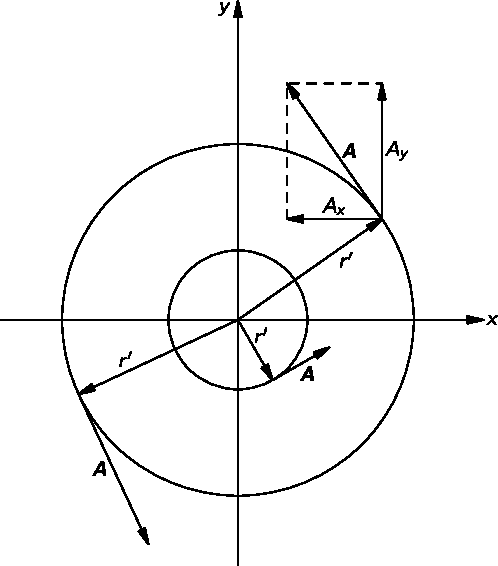
\includegraphics[width=0.7\linewidth]{fyz_fig0673.pdf}
      \caption{
               (\cite[s.~707]{Feynman02})}
      \label{fyz:fig0673}
    \end{figure}

    \begin{figure}[ht!] %\ref{fyz:fig0674}
      \centering
      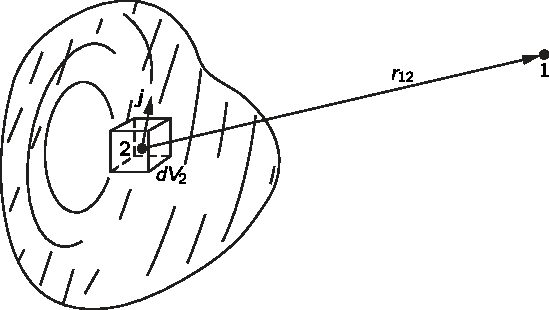
\includegraphics[width=0.7\linewidth]{fyz_fig0674.pdf}
      \caption{
               (\cite[s.~707]{Feynman02})}
      \label{fyz:fig0674}
    \end{figure}

    \begin{figure}[ht!] %\ref{fyz:fig0675}
      \centering
      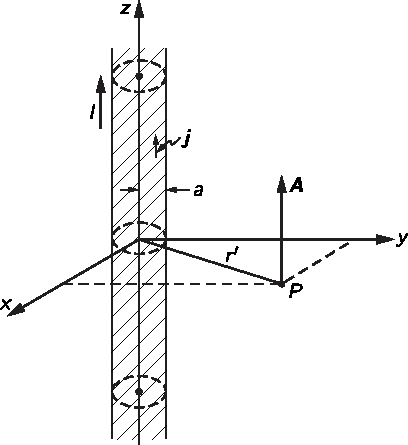
\includegraphics[width=0.7\linewidth]{fyz_fig0675.pdf}
      \caption{
               (\cite[s.~707]{Feynman02})}
      \label{fyz:fig0675}
    \end{figure}

    \begin{figure}[ht!] %\ref{fyz:fig0676}
      \centering
      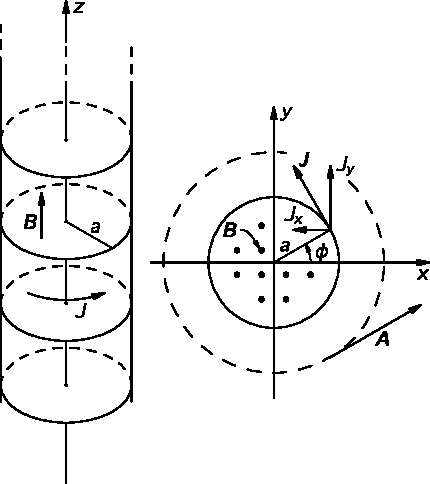
\includegraphics[width=0.7\linewidth]{fyz_fig0676.pdf}
      \caption{
               (\cite[s.~707]{Feynman02})}
      \label{fyz:fig0676}
    \end{figure}
    
    \begin{figure}[ht!] %\ref{fyz:fig0677}
      \centering
      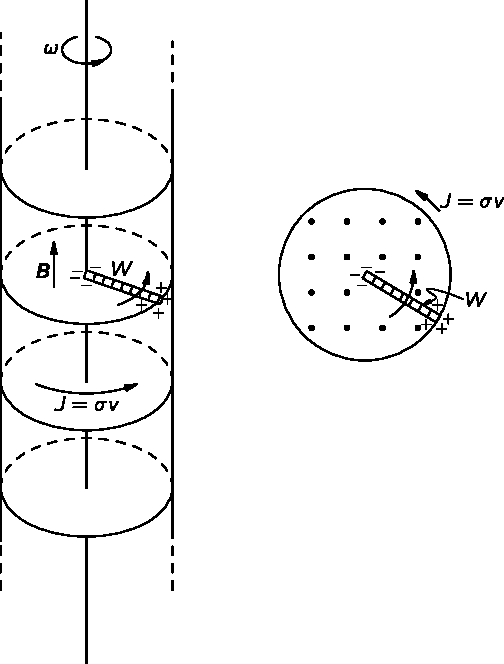
\includegraphics[width=0.7\linewidth]{fyz_fig0677.pdf}
      \caption{
               (\cite[s.~707]{Feynman02})}
      \label{fyz:fig0677}
    \end{figure}

    \begin{figure}[ht!] %\ref{fyz:fig0678}
      \centering
      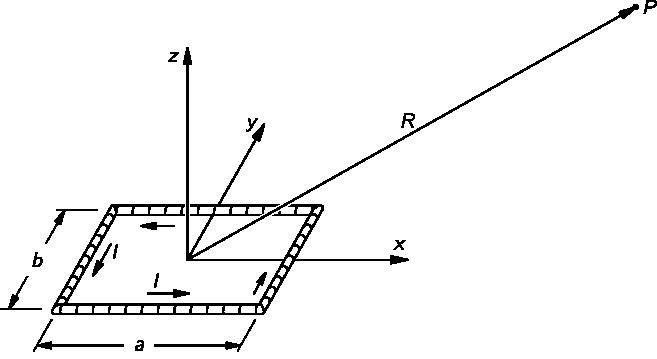
\includegraphics[width=0.7\linewidth]{fyz_fig0678.pdf}
      \caption{
               (\cite[s.~707]{Feynman02})}
      \label{fyz:fig0678}
    \end{figure}

    \begin{figure}[ht!] %\ref{fyz:fig0679}
      \centering
      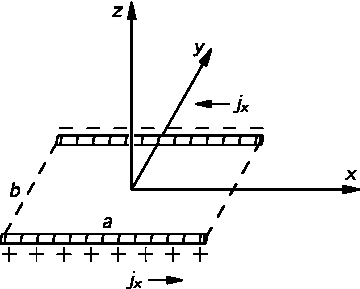
\includegraphics[width=0.7\linewidth]{fyz_fig0679.pdf}
      \caption{
               (\cite[s.~707]{Feynman02})}
      \label{fyz:fig0679}
    \end{figure}

    \begin{figure}[ht!] %\ref{fyz:fig0680}
      \centering
      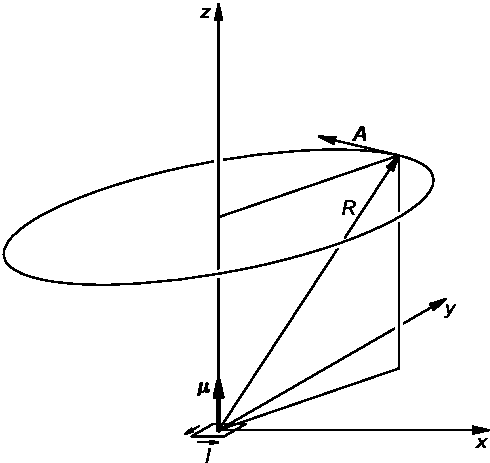
\includegraphics[width=0.7\linewidth]{fyz_fig0680.pdf}
      \caption{
               (\cite[s.~707]{Feynman02})}
      \label{fyz:fig0680}
    \end{figure}

    \begin{figure}[ht!] %\ref{fyz:fig0681}
      \centering
      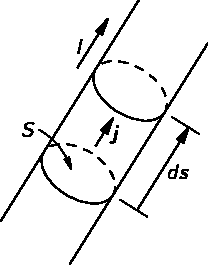
\includegraphics[width=0.5\linewidth]{fyz_fig0681.pdf}
      \caption{
               (\cite[s.~707]{Feynman02})}
      \label{fyz:fig0681}
    \end{figure}

    \begin{figure}[ht!] %\ref{fyz:fig0682}
      \centering
      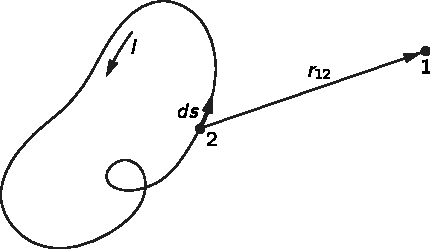
\includegraphics[width=0.7\linewidth]{fyz_fig0682.pdf}
      \caption{
               (\cite[s.~707]{Feynman02})}
      \label{fyz:fig0682}
    \end{figure}


    \todo[inline]{Kapitola fey2ch14 je nedodělaná, obsahuje pouze obrázky}
%} %tikzset
%~~~~~~~~~~~~~~~~~~~~~~~~~~~~~~~~~~~~~~~~~~~~~~~~~~~~~~~~~~~~~~~~~~~~~~~~~~~~~~~~~~~~~~~~~~~~~~~~~~
